
\chapter{Design of Module \textit{threads}}


\section{Initial Functionality}

Describe briefly what you have been given (have started from) at the beginning of the assignment and the way the existing functionality must be extended.

\section{Data Structures and Functions}

Specify the \textit{data structures} and \textit{functions} involved in your solution and what are they used for. Describe in few words the purpose of new added data structures, fields and functions. 

\begin{lstlisting}
	struct existent_data_structure {
		int newField;
	};
	
	struct newDataStructure {
	};
	
	int newFunction();
\end{lstlisting}


\section{Functionality}

Describe \textbf{briefly}, still \textbf{explicitly}, in words and pseudocode the way your solution works. DO NOT INCLUDE detailed code. 

Give examples, if you think they can make your explanation clearer. You are free to use any other techniques (e.g. use-case diagrams, sequence diagrams etc.) that you think can make your explanation clearer. See Figure~\ref{fig:sample-image} below to see the way images are inserted in a Latex file. 

\begin{figure}[h]
	\centering
	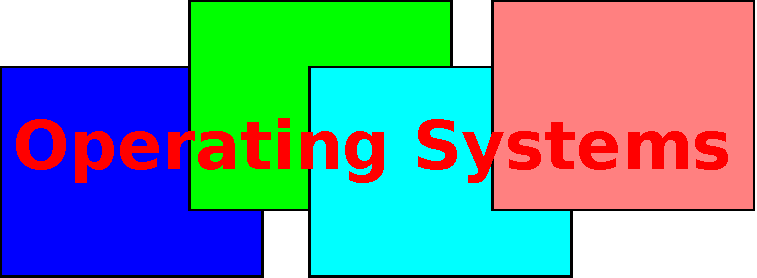
\includegraphics[width=0.5\textwidth]{figures/sample-image.pdf}
	\caption{Sample image}
	\label{fig:sample-image}
\end{figure}


Here you have a pseudo-code description of an algorithm taken fom \\ \href{http://en.wikibooks.org/wiki/LaTeX/Algorithms\_and\_Pseudocode\#Typesetting\_using\_the\_program\_package}{http://en.wikibooks.org/wiki/LaTeX}. It uses the \textit{program} package. Alternatively, you can use \textit{algorithmic} or \textit{algorithm2e} packages. 

\begin{program}
\mbox{Example of a pseudo-code algorithm description:}
\BEGIN %
  \FOR i:=1 \TO 10 \STEP 1 \DO
     |expt|(2,i); \\ |newline|() \OD %
\rcomment{This text will be set flush to the right margin}
\WHERE
\PROC |expt|(x,n) \BODY
          z:=1;
          \DO \IF n=0 \THEN \EXIT \FI;
             \DO \IF |odd|(n) \THEN \EXIT \FI;
\COMMENT{This is a comment statement};
                n:=n/2; x:=x*x \OD;
             \{ n>0 \};
             n:=n-1; z:=z*x \OD;
          |print|(z) \ENDPROC
\END
\end{program}


\section{Design Decisions}

Justify your design decisions, specify other design alternatives, their advantages and disadvantages and mention the reasons of your choice.  

\section{Tests}

Describe briefly the tests you are intended to run in order to test the functionality of your implementation.

\section{Observations}

You can use this section to mention other things not mentioned in the other sections. 

You can indicate and evaluate, for instance:
\begin{itemize}
	\item the most difficult parts of your assignment and the reasons you think they were so; 
	
	\item the difficulty level of the assignment and if the allocated time was enough or not; 

	\item particular facts or hints you think we should students to help them solve better the assignment.

\end{itemize}

You can also make suggestions for teacher, relative to the way he can assist more effectively the students.
